\documentclass[a4paper, 12pt]{report}
\usepackage[margin=1in]{geometry}
\usepackage{graphicx}
\usepackage{amsmath}
\usepackage{tikz}
\usepackage{circuitikz}
\usepackage[parfill]{parskip}
\usepackage{lipsum}
\usepackage{todonotes}
\usepackage{float}
\usepackage{subcaption}
\usepackage{plantuml}
\usepackage{hyperref}
\usepackage{array}
\hypersetup{
    colorlinks=true,
    linkcolor=black,
    urlcolor=blue
}

\title{Vacuum Robot \\  \large Semester Project Report \\ BEng-8D}
\author{
    Lukas Pillibeit \\
    Luis Manso Velasco \\
    Jessica Gomes Tavares \\
    Alain Ordoñez Ibarra \\
    Gabriele Gandolfo \\
    Francisco Javier Calles Ortega \\
    \\
    \\
    Bachelor of Engineering \\
    Semester 3 \\
    SPRO3 \\
    23.12.2026
         }
\date{May 2026}

\begin{document}

\maketitle

\pagenumbering{roman}
\tableofcontents
\listoffigures
\listoftables
\clearpage

\pagenumbering{arabic}

\chapter{Introduction}
\section{Background and Motivation}
Introduce the project context, why the problem matters, 
and the motivation for undertaking the project.

3D - Introduce the practical context in which the proposed product or system will be used. 
Describe the user, stakeholder, application, or operational problem that creates the need 
for the project. Explain why existing products, processes, or solutions do not adequately meet that need.

\section{Market Analysis}
Identify target users or customers, user needs, existing products or 
solutions, competitors, market trends, and the market gap addressed 
by the project.

Our vacuum cleaner is primarily aimed at the european market. Therefore, the
following analysis is based surveys and predictions done on this market only, unless
otherwise specified.
\subsection{Projected Market Size and Growth}
According to a report by data bridge market research, the current robotic vacuum
cleaner market in Europe has a market size of about 1.65 billion $USD$ with a
compounding annual growth Rate (CAGR) of around 10 \% to a market size of around
3.39 billion $USD$\nomenclature{$USD$}{ United States Dollar} in 2032.\cite{market_analysis_1}

\begin{figure}[H]
    \centering
    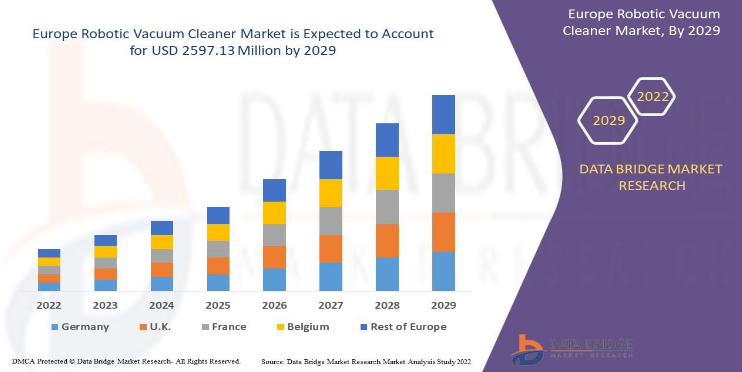
\includegraphics[width=0.7\textwidth]{images/market_analysis_1.png}
     \caption{Expected growth of the european market until 2032}
    \label{fig:marketanalysis_1}
\end{figure}

These numbers clearly indicate a flourishing market with lots of growth potential.
Out of all the robotic cleaners, the vacuuming floor robot is the most in demand and has
the biggest market share out of all the options.\cite{market_analysis_2}

\begin{figure}[H]
    \centering
    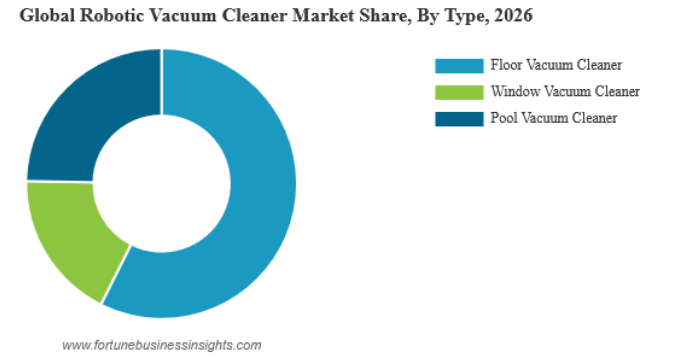
\includegraphics[width=0.7\textwidth]{images/market_analysis_2.png}
     \caption{Global Market Vacuum Cleaner Market Share}
    \label{fig:marketanalysis_2}
\end{figure}

\subsection{Most in demand robot type}
Another survey done by fortune also came to the conclusion that the robot type most in
demand is the class of robots below 150 $USD$.\cite{market_analysis_3}
Since we are building a prototype with a budget of 2000 $DKK$\nomenclature{$DKK$}{Danish Crowns} (around 300 USD), we are
confident that a successful prototype would mean that the final product is in this exact price category.


\subsection{User Analysis}
The primary target group for this vacuum robot prototype consists of young
professionals (aged 24–35) living in urban apartments ranging from 50 to 90 $m^2$. This
demographic is characterized by:

\begin{itemize}
    \item Demanding work schedules leaving less free time and consequently desiring an effortless way to clean the house without spending personal time on chores.
    \item High digital literacy, thus expecting everything to be operable via an app.
    \item Price sensitivity: possessing a limited budget and income and seeking an economical price point while still providing all essential functions.
\end{itemize}

As a result, our target group wants a straightforward way to keep their apartment clean
without investing their own time.
We are focusing on the bare minimum of cleaning functionality to keep costs as low as
possible, while still delivering necessary features (vacuuming and obstacle navigation)
and omitting luxury extras like self-emptying stations or camera recognition.
Since we can expect our demographic to be relatively digitally adept, we are integrating
numerous functions—such as starting and stopping the robot—into a mobile
application. This approach appeals directly to the consumer and allows us to turn
hardware constraints into smart software solutions.
\section{Problem Formulation}
State the central engineering problem or research question. 
The formulation should be specific enough to guide design 
decisions and evaluation.

\subsection{Problem Statement}
Write one clear question or statement describing what must 
be designed, developed, investigated, or validated. 

\subsection{Requirements}
Define functionality, performance, user, safety, reliability, 
environmental, cost, and regulatory requirements where relevant.

\subsection{Specifications}
Translate requirements into measurable targets and state how each target will be verified.

\begin{center}
    \begin{tabular}{| c | c | c | c |}
        \hline
        ID & Requirement & Specification / Target & Verification Method \\
        \hline 
    \end{tabular}
\end{center}
\section{Scope and Limitations}
Define what is included, what is excluded, the project constraints.
\section{Risk Analysis}
Identify technical, project, safety, cost, schedule, 
and implementation risks. Explain practical mitigation measures.

\chapter{Methodology}

\section{Project Approach}
Describe the overall research or engineering approach, the main stages of the project, 
and how these stages support problem formulation. Explain how different mechanical 
topologies and electrical/electronic techniques are identified, evaluated, and 
selected. Describe how interactions, dependencies, and trade-offs between the different 
domains (e.g., mechanical and electronics) are considered when developing the integrated 
mechatronic system. 
\section{Methods and Tools}
Identify the analytical, modelling, simulation, 
experimental, or design methods used. Identify 
relevant software, equipment, and other tools used. 
\section{Data Collection and Analysis}
Explain what data or evidence will be collected or generated, 
how sources or samples are selected, and how the data will be 
processed and analyzed.
\section{Verification and Validation Strategy}
Define how the proposed solution or investigation 
will be evaluated against the requirements, specifications, 
and problem formulation. 

\chapter{Design and Development}
Explain how a solution was developed to meet the requirements and specifications. 

\section{Concept Generation}
Present the concepts or technical approaches considered.
\section{Concept Evaluation and Seletion}
Explain trade-offs and justify the final selection. 
\section{System Design}
Present the overall architecture and the relevant mechanical, 
electronic, software, control, interface, material, and component design. 
\section{Engineering Analysis}
Include the calculations, modelling, simulation, dimensioning, 
component selection, control analysis, and uncertainty analysis that 
support the design. 
\section{Prototype / Implementation}
Describe manufacturing, software implementation, 
assembly, integration, and the realised prototype.

\chapter{Results}
Present the final tests, measured results, verification, and interpretation.

\section{Experimental / Test Setup}

Describe procedures, test conditions, measurements, 
number of trials, and reference or ground truth.
\section{Results}
Present measurements, graphs, tables, photographs, simulation 
outputs, and performance metrics objectively.
\section{Verification of Requirements and Specification}
Compare every measurable target from Section 1.3 with the achieved result.

\begin{center}
    \begin{tabular}{| c | c | c | c | c | }
        \hline
        ID & Specification & Target & Achieved Result & Status \\
        \hline
    \end{tabular}
\end{center}
\section{Discussion}
Interpret the results. Discuss expected and unexpected behaviour, design strengths
and weaknesses, errors, uncertainty, repeatability, 
limitations, and comparison with existing solutions.

\chapter{Conclusion and Future Work}
Close the report by answering the problem formulation and identifying justified next steps.

\section{Conclusion}

State what was developed,
the achieved performance, which requirements were met or not met, 
and whether the overall problem was solved. 
\section{Future Work}
Prioritise concrete next steps: must fix, should improve, and could develop.


\clearpage

\bibliographystyle{unsrturl}
\bibliography{refs/refs}

\clearpage

State whether AI tools were used in preparing the project/report.
If used, briefly identify the tool(s), describe how they were used,
and clarify how the generated output was reviewed, verified, and incorporated into the work.

\appendix

\end{document}